\documentclass[letterpaper, 10pt,titlepage]{article}

\usepackage[utf8]{inputenc}
\usepackage [english]{babel}
\usepackage [autostyle, english = american]{csquotes}
\usepackage{graphicx}                                        
\usepackage{amssymb}                                         
\usepackage{amsmath}                                         
\usepackage{amsthm}                                          
\usepackage{alltt}                                           
\usepackage{float}
\usepackage{url}
\newcommand\tab[1][1cm]{\hspace*{#1}}
\setlength{\parindent}{0em}
\setlength{\parskip}{1em}
\usepackage{pst-gantt}
\usepackage[letterpaper, margin=0.75in]{geometry}
\usepackage{balance}
\usepackage[TABBOTCAP, tight]{subfigure}
\usepackage{enumitem}
\usepackage{pstricks, pst-node}
\usepackage{hyperref}
\hypersetup{
  colorlinks = true,
  linkcolor  = black
}
\usepackage{listings}
\usepackage{color}
 
\definecolor{codegreen}{rgb}{0,0.6,0}
\definecolor{codegray}{rgb}{0.5,0.5,0.5}
\definecolor{codepurple}{rgb}{0.58,0,0.82}
\definecolor{backcolour}{rgb}{0.95,0.95,0.92}
 
\lstdefinestyle{mystyle}{
    backgroundcolor=\color{backcolour},   
    commentstyle=\color{codegreen},
    keywordstyle=\color{magenta},
    numberstyle=\tiny\color{codegray},
    stringstyle=\color{codepurple},
    basicstyle=\footnotesize,
    breakatwhitespace=false,         
    breaklines=true,                 
    captionpos=b,                    
    keepspaces=true,                 
    numbers=left,                    
    numbersep=5pt,                  
    showspaces=false,                
    showstringspaces=false,
    showtabs=false,                  
    tabsize=2
}
 
\lstset{style=mystyle}
\usepackage{minted}




\setcounter{secnumdepth}{4}
\def\name{Jiawei Liu}

\hypersetup{
  colorlinks = true,
  urlcolor = black,
  pdfauthor = {\name},
  pdfkeywords = {Problem Statement},
  pdftitle = {Capstone Project},
  pdfsubject = {Capstone Project},
  pdfpagemode = UseNone
}



\begin{document}

\begin{titlepage}
\begin{center}
    \Huge
    \textbf{Winter Midterm Progress Report}\\
    \textbf{Capstone Project}\\
    \vspace{1.0cm}
    \large
    Developers: Charles Henninger, Duncan Millard, Jiawei Liu\\
    Sponsor: Nancy Hildebrandt\\
    \vspace{1.5cm}
    \large
    Instructor: D. Kevin McGrath\\

    \large
    CS 462, Winter 2017, Oregon State University\\    

    \vspace{3.2cm}

    \large
    \underline{Abstract}\\
    \vspace{0.3cm}
    \end{center}
    \large

    \tab The Santiam wagon trail is historic trail located in the Willamette National Forest. The local ranger stations wish to have a mobile app that is capable of taking users on a tour of the wagon trail without needing a connection to the internet. The mobile application come in two forms: one developed for the Android mobile platform, and the other developed for the iOS mobile platform. While these two forms of the mobile application will be developed separately, they will be using the same methods of providing a tour to the user. The mobile application will render a map using a pre-downloaded map tile file and place waypoints onto the map that will be related to relevant information, in the form of videos and text files, about that area of the map. In order to achieve this functionality without internet access, we will rely on pre-downloaded content packs that will contain the map tiles, videos, text files, and waypoint information. These content packages will be created by staff of the local ranger stations, and uploaded via a website that will be developed along with the mobile app. Our team will divide these three larger sections of this project (the Android application, iOS application, and the Web Control panel/backend engineering) between the team members as follows: Android application development: Charles Henninger, Web Control panel/backend engineering: Duncan Millard, iOS application development: Jiawei Liu. This document outlines the possible technologies that will be used to address problems in each of these three major development sections, written by the team member heading each of the sections.
    
    \vspace{0.8cm}
    \vfill
    
\begin{center}    
    Feb 17, 2016

\end{center}
\end{titlepage}


\tableofcontents
\newpage



\section{Introduction}
\subsection{Team number and project name}
We are group \#43, and project name is Santiam Wagon Trail Mobile App.


\subsection{Team members and role in the project}
Jiawei Liu: The role as a UI designer which work on iOS UI, Web Control Panel UI, and Remote API Interactions. \\
Charles Henninger: Android UI Design and Functionality, Map Rendering, Android Remote API Interactions\\
Duncan Millard: Web Control Panel functionality, Inter-App framework


\vspace{0.3cm}




\section{Jiawei Liu's Section}

\subsection{iOS App Development}
This project is going to develop iOS and Android map, then offer a web control panel to manage waypoints. In detail, this project will include a mobile application (iOS and Android), the Trail Companion, that will work with custom content packages downloaded in the app. A website will be included for administrators to upload content packages to a server where the application then request and download the packages. The mobile application will provide the user with an interactive map of an area, the user’s location, and waypoints on within the area containing information about the park. This application will require no Internet access after downloading the content packages and application itself.
 
Currently, I am working on the iOS app for our project. I finished the basic UI and include all setting options in the page such as silent mode, app version, credits and help page. As screenshots show, the home page will be “My Tours” and display the map, waypoints and user’s location. Then, there are four subpages when the user click menu button, which are My Tours, Discover, Setting and Help. Now the setting page and help page are ready for use.
 
The next step of iOS app development is read waypoints and download the content package from our server. In the rest of this term, I will mainly work on the connection between server and iOS app. For example, read the available region, show waypoints on the map, and load detail description from the content package.
 
During the iOS app development, the major problem is nobody familiar with iOS development, and OSU doesn’t teach iOS development. And then, iOS using Swift to develop apps, so I need to learn a new language to develop the iOS app. Our group decides to use Android style slider menu as our app’s UI, but this is not the default iOS UI, I will include extra style file to achieve it. In addition, Xcode doesn’t like Android Studio, it only works on Mac OS system. For the map, since most map providers charge for using offline map, we also did some research for the map provider to avoid charging.
 
For solving above problems, I begin to learn how to develop iOS app on the Internet. There are some good tutorials on YouTube and Apple website to help me begin the project. Since I can find some useful tutorials on the Internet, so it solved the problem that nobody familiar with iOS development. For learning swift, I found a website called “runoob.com”, this website provides a helpful tutorial for swift, I learn the basic knowledge of swift programming during the winter break. For the UI, since Xcode didn’t include this UI template, so I google how to design slide bar in iOS. Fortunately, I found a great tutorial about how to create a slider menu on iOS, which is “ashishkakkad.com”. Then I use this tutorial as the template to develop our project. Since I am the only person that owns a Mac device in our group, I decide to work on iOS app development. For the map provider, since Mapbox can provide free offline map and customized map. We choose Mapbox as the map provider and the default map framework.
 
For solving above problems, I start to learn how to develop iOS app on the Internet. There are some good tutorials on YouTube and Apple website to help me begin the project. Since I can find some useful tutorials on the Internet, so it solved the problem that nobody familiar with iOS development. For learning swift, I found a website called “runoob.com”, this website provides a good tutorial for swift, I learn the basic knowledge of swift programming during the winter break. For the UI, since Xcode didn’t include this UI template, so I google how to design slide bar in iOS. Fortunately, I found a great tutorial about how to create slide menu on iOS, which is “ashishkakkad.com”. then I use this tutorial as the template to develop our project. Since I am the only person that own a Mac device in our group, I decide to work on iOS app development. For the map provide, Since Mapbox can provide free offline map and customized map. We choose Mapbox as the map provider and default map framework. In addition, Mapbox has a detailed tutorial to teach me how to include the map in the iOS app and display waypoints.

According to thefreedictionary.com, the definition of experimental design is “research design that eliminates all factors that influence outcome except for the cause being studied (independent variable). All other factors are controlled by randomization, investigator-controlled manipulation of the independent variable, and control of the study situation by the investigator, including the use of control groups. [1]” In my opinion, experimental design is useful for our project, it can improve our design and provide a more comfortable user experience. For example, I can design an experiment to test user map preference in many ways. I can download couples of maps app such as Google Map, Here Map, and Open Street Map. We can observe users’ habit and summary their preference. Then we can optimize our app UI and provide a better user experience.
 
For the interface design, we discussed the UI design as a group and our group member Charles did a great app UI paper prototypes, then uploaded to our group GitHub. We use this paper prototype as the reference to develop our project. I hope users are going to click the waypoint and understand how to visit the waypoint when the first time they use this app. In addition, Since I used the Android style slider menu, it is popular in Android but not in iOS, I hope users can click the menu button to check more features.
 
For the screenshots, I have six screenshots, which are home page, slider menu, setting page, help page, Xcode and Storyboard at the bottom of report. 


\subsection{Swift Code for Slider Menu}
\begin{minted}{swift}
import UIKit

protocol SlideMenuDelegate {
    func slideMenuItemSelectedAtIndex(_ index : Int32)
}

class MenuViewController: UIViewController, UITableViewDataSource, UITableViewDelegate {

    @IBOutlet var tblMenuOptions : UITableView!
    
    @IBOutlet var btnCloseMenuOverlay : UIButton!

    var arrayMenuOptions = [Dictionary<String,String>]()
    var btnMenu : UIButton!
    var delegate : SlideMenuDelegate?
    
    override func viewDidLoad() {
        super.viewDidLoad()
        tblMenuOptions.tableFooterView = UIView()
        // Do any additional setup after loading the view.
    }
    
    override func didReceiveMemoryWarning() {
        super.didReceiveMemoryWarning()
        // Dispose of any resources that can be recreated.
    }
    
    override func viewWillAppear(_ animated: Bool) {
        super.viewWillAppear(animated)
        updateArrayMenuOptions()
    }
    
    func updateArrayMenuOptions(){
        arrayMenuOptions.append(["title":"My Tours", "icon":"HomeIcon"])
        arrayMenuOptions.append(["title":"Discover", "icon":"PlayIcon"])
        arrayMenuOptions.append(["title":"Setting", "icon":"SettingIcon"])
        arrayMenuOptions.append(["title":"Help", "icon":"HelpIcon"])
        
        tblMenuOptions.reloadData()
    }
    
    @IBAction func onCloseMenuClick(_ button:UIButton!){
        btnMenu.tag = 0
        
        if (self.delegate != nil) {
            var index = Int32(button.tag)
            if(button == self.btnCloseMenuOverlay){
                index = -1
            }
            delegate?.slideMenuItemSelectedAtIndex(index)
        }
        
        UIView.animate(withDuration: 0.3, animations: { () -> Void in
            self.view.frame = CGRect(x: -UIScreen.main.bounds.size.width, y: 0, width: UIScreen.main.bounds.size.width,height: UIScreen.main.bounds.size.height)
            self.view.layoutIfNeeded()
            self.view.backgroundColor = UIColor.clear
            }, completion: { (finished) -> Void in
                self.view.removeFromSuperview()
                self.removeFromParentViewController()
        })
    }
    
    func tableView(_ tableView: UITableView, cellForRowAt indexPath: IndexPath) -> UITableViewCell {
        let cell : UITableViewCell = tableView.dequeueReusableCell(withIdentifier: "cellMenu")!
        
        cell.selectionStyle = UITableViewCellSelectionStyle.none
        cell.layoutMargins = UIEdgeInsets.zero
        cell.preservesSuperviewLayoutMargins = false
        cell.backgroundColor = UIColor.clear
        
        let lblTitle : UILabel = cell.contentView.viewWithTag(101) as! UILabel
        let imgIcon : UIImageView = cell.contentView.viewWithTag(100) as! UIImageView
        
        imgIcon.image = UIImage(named: arrayMenuOptions[indexPath.row]["icon"]!)
        lblTitle.text = arrayMenuOptions[indexPath.row]["title"]!
        
        return cell
    }
    
    func tableView(_ tableView: UITableView, didSelectRowAt indexPath: IndexPath) {
        let btn = UIButton(type: UIButtonType.custom)
        btn.tag = indexPath.row
        self.onCloseMenuClick(btn)
    }
    
    func tableView(_ tableView: UITableView, numberOfRowsInSection section: Int) -> Int {
        return arrayMenuOptions.count
    }
    
    func numberOfSections(in tableView: UITableView) -> Int {
        return 1;
    }
}

\end{minted}


\vspace{0.5cm}


\section{Charles Henninger's Section}
\subsection{Android App Development}
The mobile application that we are developing for the Sweet Home Ranger District of the Willamette National Forest must be developed with the capability to provide the required services without the need to connect to the internet. The application will be able to provide an interactive map that provides the user with their current location on a trail, as well as waypoints that provide information about points of interest along the trail in the form of videos, audio recordings, and text articles. Ranger Station staff must also be able to design and publish new events through a website with little technical knowledge. Finally, this project must have minimal recurring costs, and must be available for both iOS and Android devices. The relevant viewpoints that we will be concerning with for this project are that of the developers, the administrators, and the users. We will take into account these viewpoints when designing our solutions to each of the requirements, and mold our design in accordance with what is best for each point of view. 

Current progress of our application extends to our alpha prototype, which includes an Android and iOS user interface and the basic structure of our server planned out. The Android user interface will be implementing the paper prototype of the general user interface that our group created. At this stage in development our user interface contains a menu allowing navigation between the different pages of the application, a page containing a interactive mapbox mapview object, and a unique launch icon that will be the main logo of the application. 

Most of the work that went into the development of the Android user interface for the alpha version of our application was centered around how the different features of the application were to be implemented later in the design process. The decision was between a single Android Activity (serving as the navigation drawer for the rest of the app) implementing many different Fragments, or having many Android Activities that the application would switch between. This design decision was one of the first major problems that we faced in development, and eventually came down to the compatibility of Mapbox (the third party software that we are using to render our maps) with Android Fragments. Implementing a Mapbox map on an Android Fragment is possible, but sacrifices a lot of the versatility of the Mapbox software to do so. Due to this, the decision was made to organize the application into many Android Activities that were extensions of the main Navigation menu Activity, thereby allowing the app to run many Activities and maintain access to an overarching Activity with handles navigation between them. The first step in this process was to create Activities for the Settings, Help, My Tours, and Discovery sections of our application that were descended from a generic Navigation Drawer Activity. In the Navigation Drawer Activity we created an overridden setContentView method that the other activities would call on creation, while passing the view id for their specific XML file. The Navigation Drawer Activity then inflates that Activity's XML layout inside a blank Framelayout located in it's XML file, right above the code for the Navigation Drawer. By doing this, we create more possibilities for each Activity to have it's own set of fragments, and insure that Mapbox will be working in a way that meets the requirements of this project. 

With the general architecture of the Android application complete, attention will move to polishing the supporting features of the application (such as lists, usability settings, and Activity transitions), application aesthetics, and development of the communication between the server and the application. 

The XML and Java code for the Navigation Drawer is listed below, as well as images from our application's UI and Mapbox Map.

\subsection{Overridden Set Content View}
\begin{minted}{java}
public class Drawer extends AppCompatActivity implements NavigationView.OnNavigationItemSelectedListener {


   protected DrawerLayout fullLayout;
   protected FrameLayout frameLayout;
   @Override
   public void setContentView(int layoutResID) {

       //this appends the desired activity layout to the Drawer activity layout

       fullLayout = (DrawerLayout) getLayoutInflater().inflate(R.layout.activity_drawer, null);
       frameLayout = (FrameLayout) fullLayout.findViewById(R.id.drawer_frame);

       getLayoutInflater().inflate(layoutResID, frameLayout, true);
       super.setContentView(fullLayout);

       //The navigation bar everything from here on

       Toolbar toolbar = (Toolbar) findViewById(R.id.toolbar);
       setSupportActionBar(toolbar);

       DrawerLayout drawer = (DrawerLayout) findViewById(R.id.drawer_layout);
       ActionBarDrawerToggle toggle = new ActionBarDrawerToggle(
               this, drawer, toolbar, R.string.navigation_drawer_open, R.string.navigation_drawer_close);
       drawer.setDrawerListener(toggle);
       toggle.syncState();

       NavigationView navigationView = (NavigationView) findViewById(R.id.nav_view);
       navigationView.setNavigationItemSelectedListener(this);
   }
\end{minted}
\begin{minted}{XML}

(The XML file for the Drawer Activity. The layouts for other Activities will be inflated inside the FrameLayout located here)

<?xml version="1.0" encoding="utf-8"?>
<android.support.v4.widget.DrawerLayout xmlns:app="http://schemas.android.com/apk/res-auto"
   xmlns:android="http://schemas.android.com/apk/res/android"
   xmlns:tools="http://schemas.android.com/tools"
   android:layout_width="match_parent"
   android:layout_height="fill_parent"
   android:fitsSystemWindows="true"

   android:id="@+id/drawer_layout"
   tools:openDrawer="start">

   <include
       layout="@layout/app_bar_drawer"
       android:layout_width="match_parent"
       android:layout_height="match_parent" />

   <FrameLayout
       android:id="@+id/drawer_frame"
       android:layout_width="match_parent"
       android:layout_height="match_parent" />

   <android.support.design.widget.NavigationView
       android:id="@+id/nav_view"
       android:layout_width="wrap_content"
       android:layout_height="match_parent"
       android:layout_gravity="start"
       android:fitsSystemWindows="true"
       app:headerLayout="@layout/nav_header_drawer"
       app:menu="@menu/activity_drawer_drawer" />

</android.support.v4.widget.DrawerLayout>

\end{minted}




\vspace{0.5cm}

\section{Duncan Millard's Section}
\subsection{Overview}
While much of the work on our project solution is focused on the mobile applications, a critical aspect of the solution as a whole is our back end system. One of the original reasons for creating our project was to design a system such that Ranger staff would not need to allocate as many hours to compiling together the physical and recorded assets for seasonal Interpretive events. With the current methods, the Sweet Home Ranger staff are drafting and publishing posters and papers and then displaying them in site-specific billboards. This, along with recorded tours on cassette tapes, has a surprisingly large labor overhead for creating, deploying, and maintaining events. This said, one of the critical facets of our solution is to not just provide a user-friendly application for visitors, but to also provide a clean mechanism for managing the content published to the application.

\subsection{Server and Control Panel}
In order to accomplish this task, we have decided to have a central server provide hosting and content serving abilities to act as a virtual warehouse of pre-made tours. This warehouse will also come with a content creation interface allowing Ranger staff to create and publish new tours. This segment will describe the progress that has been made in securing hardware, its configuration, and some pitfalls encountered along the way.

In week 2 of this Winter term, our team has allocated Thursday afternoons at 14:00 to work as a unit. During these time slots, we will be taking advantage of the Capstone Lab in order to test both mobile applications and our central server at once. While we have simultaneous development across our systems, the primary blocker will be the applications requiring information from our server. As a result, I have been crafting pre-made content that can easily be emulated by our server to act in lieu of real production data.

Starting with Week 3 of this term, we received an Intel NUC as a temporary server to use for our project from Dr. McGrath. The particular NUC we are using is an i7-5557U processor variant that is more than adequate for our needs. As we move forward to actually deploying our solution, this hardware will likely be left behind. In an effort to not waste hours of configuration work, we will be delivering an RPM file containing our server deployment. This server deployment file will allow us the ‘install’ our server software onto an arbitrary internet connected Centos 7 machine. As we have chosen Centos 7, we have over 5 years of support remaining for the packages and security lifespan. From the beginning of our server setup, I have been logging the packages that we have needed to install or configure. These packages will be added to our Content Server installation process as should be installed automatically as pre-requisites for our software upon deployment.

One of the initial roadblocks that our team encountered with this server is that we were not able to hook it up arbitrarily into the OSU network. We had to request a particular Ethernet port to be allocated and opened for our own usage, as well as a hostname for our system. At the time of writing this, we have secured a home in the Capstone Lab on a dedicated Ethernet and power outlet. One issue we encountered when trying to utilize the allocated hostname was that during the Centos 7 installation, it requests a manual override for the hostname. I had entered a hostname at that time, not knowing what our eventual allocated name would be. As the allocated name is requested through DHCP, it should have taken effect immediately when IT enabled it. I had to clear the manually entered hostname before this would take effect.

In addition to requiring a hostname, we also needed the appropriate ports opened. While port 22 (SSH) was opened ahead of time, getting a port like 80 (HTTP) or 443 (HTTPS) opened within the OSU firewall is a much more risky and slow process. As a result we will be using the NodeJs suggested port of 3000 for our Web Control Panel, and port 3001 for our content package API. The need for the ports to be manually opened was discovered when we attempted to run the pair of servers on the NUC. Localhost communications worked satisfactorily, yet Flip was unable to communicate. After requesting the ports opened and opening the Centos 7 local firewall settings, we are now able to communicate with our server through these interfaces.

Beyond the basic system setup, I have started the design and implementation of our database tables. We will be using MySQL Community for Centos and have started implementing user logins and our permissions model.

Our Web Control Panel UI design has started as well. We have several bare functionality sketches that indicate a minimum viable product for our UI, drawing out our page flow and minimal functionality. We have settled currently on using JQuery for the functional aspects of the UI, with Bootstrap CSS as a responsive design webkit to enable us to take advantage of rapid development and deployment. These projects are both based on the highly permissive MIT Open Source license, which allows us to use the projects in exchange for basic citing. 


\newpage %add references at here
\begin{thebibliography}{9}

\bibitem{1} 
"thefreedictionary," \textit{thefreedictionary}. [Online]. \\Available:
\texttt{http://medical-dictionary.thefreedictionary.com/experimental+design} [Accessed: 16-Feb-2017].
%%

\end{thebibliography}



\newpage
\textbf{ }
\vspace{5.0cm}

\noindent\rule{13cm}{0.4pt}\\
Sponsor
\vspace{3.0cm}

\noindent\rule{13cm}{0.4pt}\\
Developer
\vspace{3.0cm}


\noindent\rule{13cm}{0.4pt}\\
Developer
\vspace{3.0cm}


\noindent\rule{13cm}{0.4pt}\\
Developer
\vspace{3.0cm}






\newpage
\section{Screenshots}

\begin{figure}[ht]
    \centering
    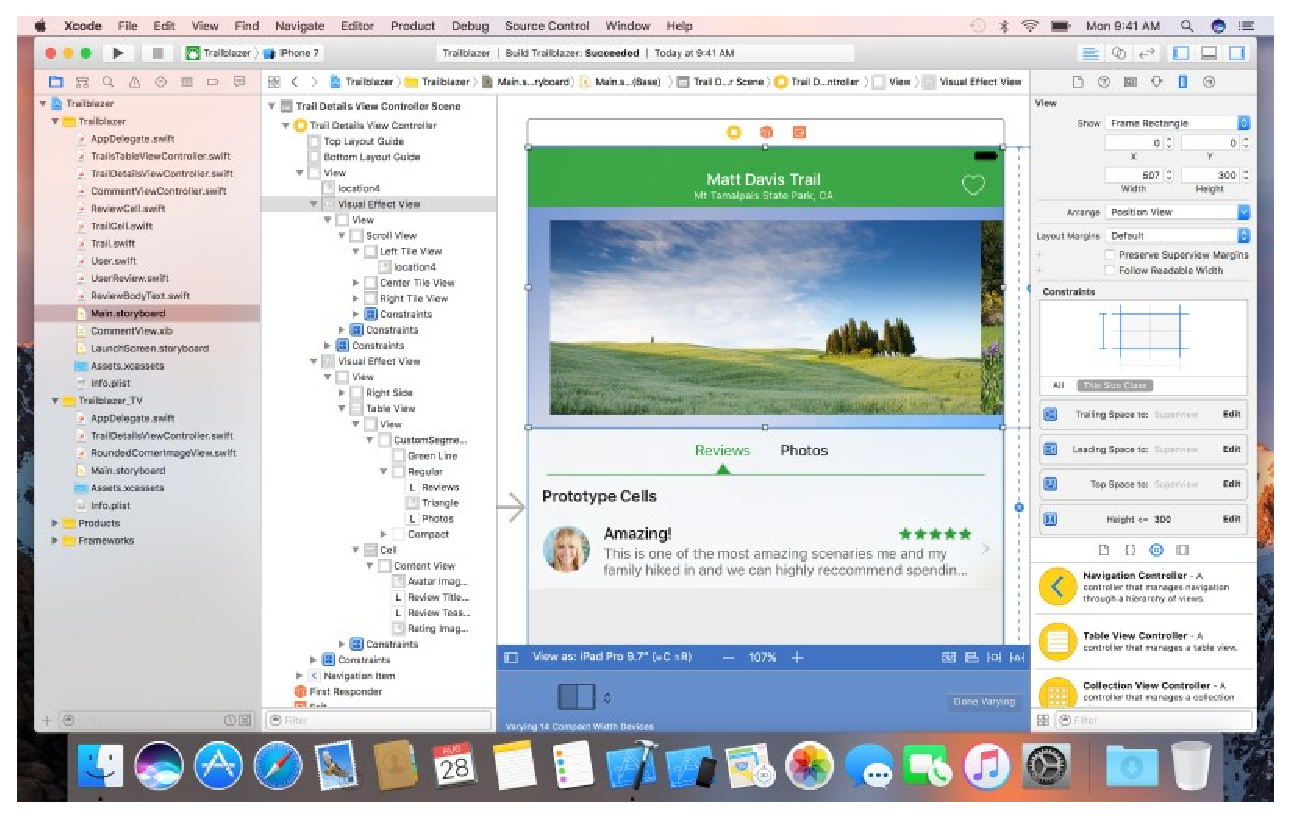
\includegraphics[scale=0.5]{j1}
    \caption{My Tours}
    \label{jiawei1}
\end{figure}

\begin{figure}[ht]
    \centering
    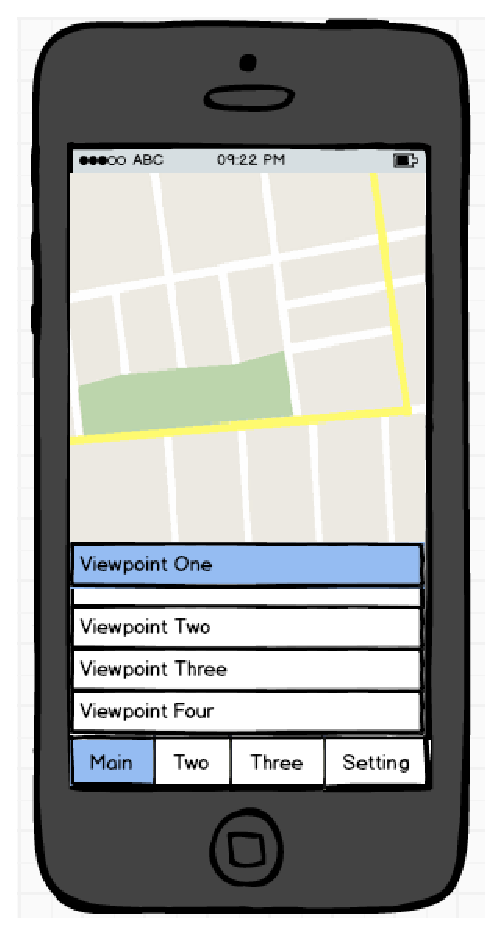
\includegraphics[scale=0.5]{j2}
    \caption{Slider Menu}
    \label{jiawei2}
\end{figure}

\begin{figure}[ht]
    \centering
    \includegraphics[scale=0.5]{j3}
    \caption{Setting}
    \label{jiawei3}
\end{figure}

\begin{figure}[ht]
    \centering
    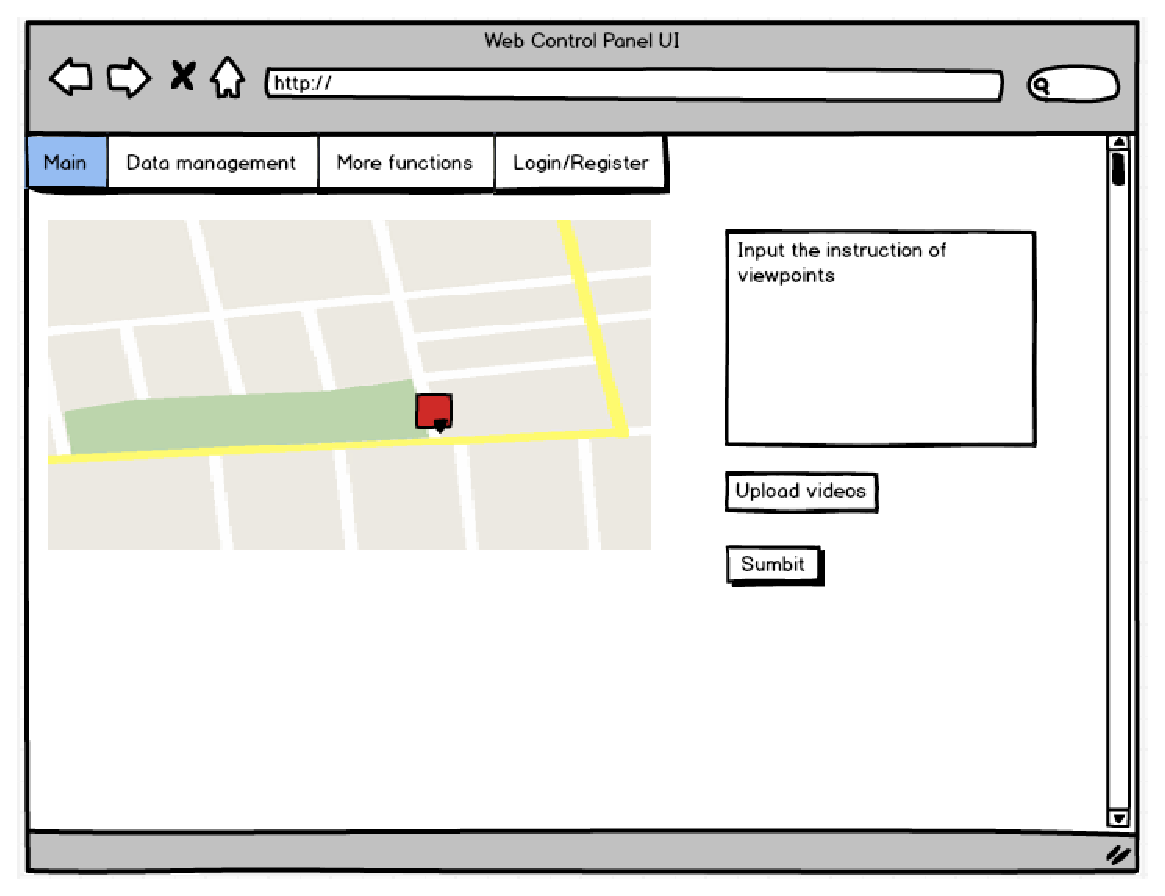
\includegraphics[scale=0.5]{j4}
    \caption{Help}
    \label{jiawei4}
\end{figure}

\begin{figure}[ht]
    \centering
    \includegraphics[width=0.8\textwidth]{j5}
    \caption{Xcode}
    \label{jiawei5}
\end{figure}

\begin{figure}[ht]
    \centering
    \includegraphics[scale=0.5]{j6}
    \caption{Storyboard}
    \label{jiawei6}
\end{figure}

\begin{figure}[ht]
    \centering
    
\includegraphics[scale=1.2]{android1}
    \caption{Android Launcher}
    \label{charles1}
\end{figure}

\begin{figure}[ht]
    \centering
    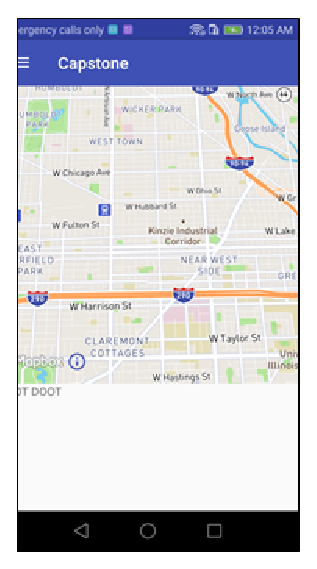
\includegraphics[scale=1.2]{android2}
    \caption{MapBox Proof of Concept}
    \label{charles2}
\end{figure}

\begin{figure}[ht]
    \centering
    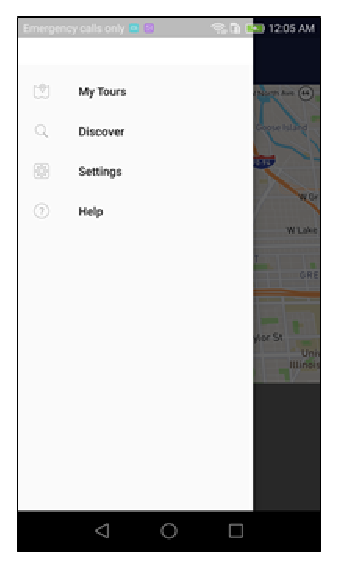
\includegraphics[scale=1.2]{android3}
    \caption{Android Drawer Menu}
    \label{charles3}
\end{figure}






\end{document}
